\documentclass[11pt]{article}

% ---------- Packages ----------
\usepackage[a4paper,margin=2.2cm]{geometry}
\usepackage{titlesec}
\usepackage{xcolor}
\usepackage{booktabs}
\usepackage{array}
\usepackage{enumitem}
\usepackage{hyperref}
\usepackage{fancyhdr}
\usepackage{parskip}
\usepackage{fontenc}
\usepackage[T1]{fontenc}
\usepackage{tikz}
\usetikzlibrary{positioning, arrows.meta, backgrounds, fit, shapes.geometric}

% ---------- Colors ----------
\definecolor{accent}{HTML}{2E4057}
\definecolor{accentlight}{HTML}{5B7B9A}

% ---------- Section styling ----------
\titleformat{\section}
  {\Large\bfseries\color{accent}}
  {\thesection}{0.6em}{}
\titleformat{\subsection}
  {\large\bfseries\color{accentlight}}
  {\thesubsection}{0.6em}{}
\titlespacing*{\section}{0pt}{1.4em}{0.8em}
\titlespacing*{\subsection}{0pt}{1.1em}{0.5em}

% ---------- Header / Footer ----------
\pagestyle{fancy}
\fancyhf{}
\renewcommand{\headrulewidth}{0.4pt}
\fancyhead[L]{\small\itshape Generative Support Agent -- Evaluation Report}
\fancyhead[R]{\small\itshape Joydeep Banik}
\fancyfoot[C]{\small\thepage}

% ---------- Hyperref ----------
\hypersetup{
  colorlinks=true,
  linkcolor=accent,
  urlcolor=accentlight,
  citecolor=accent,
  pdftitle={Generative Support Agent: Evaluation Report},
  pdfauthor={Joydeep Banik}
}

\setlist[itemize]{leftmargin=1.4em, itemsep=0.15em, topsep=0.2em}
\setlist[enumerate]{leftmargin=1.6em, itemsep=0.2em, topsep=0.2em}

\begin{document}

% ---------------- Title Page ----------------
\begin{titlepage}
\centering
\vspace*{2.5cm}
{\Huge\bfseries\color{accent} AI Customer Support Agent}\\[0.4cm]
{\Large\color{accentlight} Intent Classification, Grounded Reply Drafting, and Auto-Handle Routing for @AppleSupport}\\[2cm]

{\large\bfseries Evaluation Report}\\[0.3cm]
{\large Hiver -- SDE Intern Take-Home Assignment}\\[2.5cm]

\begin{tabular}{ll}
\textbf{Author:} & Joydeep Banik \\
\textbf{Institution:} & RCC Institute of Information Technology, Kolkata \\
\textbf{Repository:} & \url{https://github.com/Joydeep2005Banik/Hiver-SDE-Intern_Home-Assignment} \\
\textbf{Date:} & \today \\
\end{tabular}

\vfill
{\small Dataset: Customer Support on Twitter (Kaggle, thoughtvector/customer-support-on-twitter)}
\end{titlepage}

% ---------------- Section 1 ----------------
\section{Problem Framing}

\textbf{Objective.} Build a prototype generative support agent that parses incoming tweets to \texttt{@AppleSupport}, extracts the customer's underlying intent, decides whether the query can be auto-handled or needs human escalation, and drafts a polite, grounded response based on historical brand replies.

\textbf{What ``good'' means for this brand.} A good AppleSupport reply must: (1) correctly identify the customer's underlying issue, (2) resolve or meaningfully advance the conversation in a single turn (e.g.\ ask the right diagnostic question), (3) avoid hallucinating unsupported troubleshooting steps or policies, and (4) match the empathetic, professional tone Apple uses on Twitter. A reply that is polite but unhelpful, or helpful but factually wrong, is not considered good.

\textbf{What was deliberately not built.}
\begin{itemize}
  \item Multi-turn conversation tracking -- each query is treated as stateless.
  \item Sentiment-based routing -- escalation uses keyword triggers plus LLM judgement, not a dedicated sentiment model.
  \item Billing, refund, or warranty claim workflows -- these require internal system access.
  \item Proactive outreach and non-English support.
\end{itemize}

\textbf{Approach.}
\begin{enumerate}
  \item \textbf{Data-driven taxonomy:} analyzed 106k+ conversation pairs using n-gram frequency to discover nine robust intent categories (\texttt{battery\_charging}, \texttt{account\_access}, \texttt{software\_update}, etc.).
  \item \textbf{Support engine:} a \texttt{SupportAgent} that classifies intent, determines auto-handle eligibility, and drafts responses, including a contextual follow-up question or a hand-off message.
  \item \textbf{Evaluation framework:} a local harness (\texttt{evaluate.py}) that scores intent classification (accuracy/F1), auto-handle routing, and draft quality via LLM-as-a-judge (tone, helpfulness, groundedness).
\end{enumerate}

% ---------------- Section 2 ----------------
\section{System Architecture}

The pipeline has three stages: (i) data preparation and RAG index construction, (ii) the core agent that retrieves historical context and calls an LLM API to produce intent, reply, and escalation decision, and (iii) an evaluation framework that grades the agent against a hand-labelled golden set. Figure~\ref{fig:architecture} traces data and control flow across the three stages.

\begin{figure}[h]
\centering
\resizebox{\linewidth}{!}{%
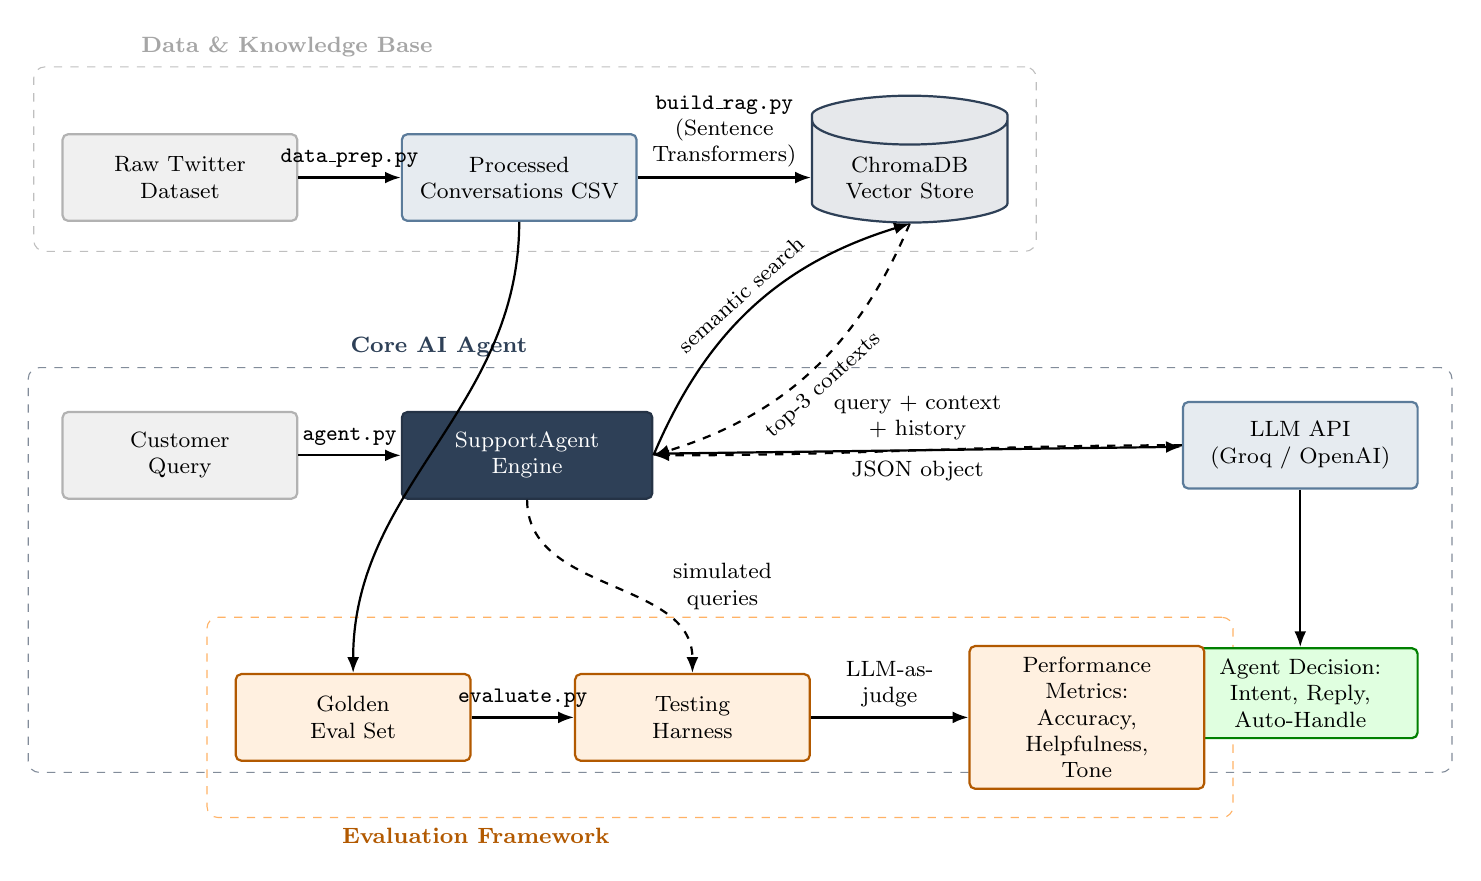
\begin{tikzpicture}[
    font=\footnotesize,
    every node/.style={align=center},
    box/.style={draw, rounded corners=2pt, minimum height=1.1cm, text width=2.7cm, inner sep=4pt, thick},
    src/.style={box, fill=gray!12, draw=gray!60},
    proc/.style={box, fill=accentlight!15, draw=accentlight},
    store/.style={box, cylinder, shape border rotate=90, aspect=0.25, fill=accent!12, draw=accent, minimum height=1.3cm, text width=2.2cm},
    engine/.style={box, fill=accent, draw=accent!80!black, text=white, text width=2.9cm},
    decision/.style={box, fill=green!12, draw=green!50!black},
    evalbox/.style={box, fill=orange!12, draw=orange!70!black},
    arr/.style={-{Latex[length=2mm]}, thick},
    darr/.style={-{Latex[length=2mm]}, thick, dashed},
    node distance=1.0cm and 1.3cm
]

% --- Row 1: Data & Knowledge Base ---
\node[src] (A) {Raw Twitter\\Dataset};
\node[proc, right=of A] (B) {Processed\\Conversations CSV};
\node[store, right=2.2cm of B] (C) {ChromaDB\\Vector Store};

% --- Row 2: Core AI Agent ---
\node[src, below=2.4cm of A] (D) {Customer\\Query};
\node[engine, right=of D] (E) {SupportAgent\\Engine};
\node[proc, right=2.2cm of C, yshift=-3.4cm] (F) {LLM API\\(Groq / OpenAI)};
\node[decision, below=2.0cm of F] (G) {Agent Decision:\\Intent, Reply,\\Auto-Handle};

% --- Row 3: Evaluation Framework ---
\node[evalbox, below=2.2cm of D, xshift=2.2cm] (H) {Golden\\Eval Set};
\node[evalbox, right=of H] (I) {Testing\\Harness};
\node[evalbox, right=2.0cm of I] (J) {Performance Metrics:\\Accuracy, Helpfulness,\\Tone};

% --- Edges: Data & Knowledge Base ---
\draw[arr] (A) -- node[above]{\texttt{data\_prep.py}} (B);
\draw[arr] (B) -- node[above, text width=2.6cm]{\texttt{build\_rag.py}\\(Sentence Transformers)} (C);

% --- Edges: Core AI Agent ---
\draw[arr] (D) -- node[above]{\texttt{agent.py}} (E);
\draw[arr] (E.east) to[bend left=25] node[midway, sloped, above]{semantic search} (C.south);
\draw[darr] (C.south) to[bend left=25] node[midway, sloped, below]{top-3 contexts} (E.east);
\draw[arr] (E) -- node[above, text width=2.6cm]{query + context\\+ history} (F);
\draw[darr] (F) to[out=180,in=0] node[below, text width=2cm]{JSON object} (E);
\draw[arr] (F) -- (G);

% --- Edges: Evaluation Framework ---
\draw[arr] (B.south) to[out=270,in=90] (H.north);
\draw[arr] (H) -- node[above]{\texttt{evaluate.py}} (I);
\draw[darr] (E.south) to[out=270,in=90] node[right, text width=2.6cm]{simulated\\queries} (I.north);
\draw[arr] (I) -- node[above, text width=2.4cm]{LLM-as-\\judge} (J);

\begin{scope}[on background layer]
\node[draw=gray!50, dashed, rounded corners, fit=(A)(B)(C), inner sep=10pt, label={[gray!70]above left:\textbf{Data \& Knowledge Base}}] {};
\node[draw=accent!60, dashed, rounded corners, fit=(D)(E)(F)(G), inner sep=12pt, label={[accent]above left:\textbf{Core AI Agent}}] {};
\node[draw=orange!60, dashed, rounded corners, fit=(H)(I)(J), inner sep=10pt, label={[orange!70!black]below left:\textbf{Evaluation Framework}}] {};
\end{scope}

\end{tikzpicture}%
}
\caption{End-to-end system architecture: data ingestion and RAG indexing, the core agent's retrieval-augmented decision loop, and the evaluation framework that grades the agent against the golden set.}
\label{fig:architecture}
\end{figure}

\begin{itemize}
  \item \textbf{Data \& knowledge base:} \texttt{src/data\_prep.py} filters the raw Twitter dataset into a processed conversations CSV; \texttt{src/build\_rag.py} embeds it with Sentence Transformers (\texttt{all-MiniLM-L6-v2}) into a ChromaDB vector store.
  \item \textbf{Core agent:} for each customer query, the \texttt{SupportAgent} retrieves the top-3 historical contexts via semantic search, sends query + context + history to the LLM API, and parses a JSON object containing intent, drafted reply, and auto-handle decision.
  \item \textbf{Evaluation framework:} the golden set is generated from processed conversations, and \texttt{evaluate.py} runs the agent against it, computing automated metrics and LLM-as-a-judge scores.
\end{itemize}

% ---------------- Section 3 ----------------
\section{Baselines and Performance}

\textbf{Golden evaluation set.} A custom 200-example golden evaluation set (\texttt{data/golden\_eval\_handlabelled.csv}) was built. It was pre-labelled using a heuristic classifier and then 100\% human-reviewed and hand-labelled, achieving a 93.5\% agreement rate with the heuristic labels.

\textbf{Baselines.} The pipeline is compared against two baselines, both computed dynamically in \texttt{src/evaluate.py}:
\begin{enumerate}
  \item \textbf{Trivial baseline (majority class):} always predicts the most common intent (\texttt{general\_inquiry}) and always predicts \texttt{auto\_handle = True}.
  \item \textbf{Simple baseline (heuristics):} uses a regex keyword matcher for intent, and sets \texttt{auto\_handle = False} for \texttt{general\_inquiry}, \texttt{True} otherwise.
\end{enumerate}

\begin{table}[h]
\centering
\begin{tabular}{lccc}
\toprule
\textbf{Metric} & \textbf{Trivial} & \textbf{Simple (Heuristics)} & \textbf{Pipeline (LLM)} \\
\midrule
Intent Accuracy      & 38.0\% & 96.5\%\textsuperscript{a} & 60.0\%\textsuperscript{b} \\
Auto-Handle Accuracy & 84.0\% & 59.0\%                     & 80.0\% \\
Draft Quality (LLM Judge) & N/A & N/A & Tone 4.0/5, Help 4.4/5, Ground 4.1/5 \\
\bottomrule
\end{tabular}
\caption{Pipeline performance vs.\ two baselines on the golden evaluation set.}
\end{table}

\footnotesize{\textsuperscript{a} The simple baseline's 96.5\% intent accuracy is artificially inflated: the golden set was initially pre-labelled using this same heuristic before human review, biasing it toward queries the heuristic already handles well.}\\
\footnotesize{\textsuperscript{b} The LLM pipeline was evaluated on a 20-sample subset to control API costs during development.}
\normalsize

\subsection{Human--LLM Agreement (Cohen's Kappa)}
Evaluated on 20 examples:
\begin{itemize}
  \item \textbf{Tone:} $\kappa = 0.000$ (degenerate -- humans scored 5/5 uniformly; the LLM judge averaged 4.0/5).
  \item \textbf{Helpfulness:} $\kappa = 0.000$ (degenerate -- humans scored 5/5 uniformly; the LLM judge averaged 4.4/5).
  \item \textbf{Groundedness:} $\kappa = 0.003$ (slight -- humans found hallucinated policies that the LLM judge missed).
\end{itemize}

% ---------------- Section 4 ----------------
\section{Failure Analysis}

\textbf{Where the system performs as expected.} It handles structured queries with clear keywords well (e.g.\ ``my battery drains fast'', ``wifi won't connect''), and correctly flags highly negative sentiment (e.g.\ explicit profanity) to force escalation.

\textbf{Top five failure modes.}

\begin{enumerate}
  \item \textbf{Hidden context (missing images/media).} Example: a customer reports their iPhone frozen for hours. Hypothesis: the customer likely attached an image or video, but the dataset is text-only, so the agent sees a generic inquiry and attempts to auto-handle what a human would escalate.
  \item \textbf{Profanity and high emotion (escalation misses).} Example: creative, non-explicit swearing expressing frustration. Hypothesis: explicit profanity triggers escalation, but stylized or disguised swearing is sometimes misclassified as standard feedback, producing an inappropriately cheerful automated reply.
  \item \textbf{Ambiguous feature vs.\ bug classification.} Example: a customer describing an SOS feature triggering unexpectedly. Hypothesis: keyword overlap with ``new feature'' causes misclassification as \texttt{software\_update} rather than \texttt{app\_bug\_crash}; keyword heuristics fail on descriptive, conversational bug reports.
  \item \textbf{Misinterpreting literal strings vs.\ grammar.} Example: a customer asking how to fix autocorrect changing ``it'' to ``I.T.''. Hypothesis: the agent classifies this as \texttt{general\_inquiry} instead of \texttt{keyboard\_typing}, since standard tokenization struggles to distinguish the literal string from the pronoun.
  \item \textbf{Multi-step conversational context loss.} Example: a mid-thread reply describing touch-screen calibration behavior. Hypothesis: this is clearly a continuation of a \texttt{hardware\_repair} thread, but the stateless agent receives only the single message and misclassifies it as \texttt{general\_inquiry}.
\end{enumerate}

% ---------------- Section 5 ----------------
\section{What Is Misleading About the Headline Numbers}

\begin{itemize}
  \item \textbf{Over-representation of ``general inquiry''.} The taxonomy covers roughly 60\% of specific issues, so about 40\% of queries fall into the \texttt{general\_inquiry} bucket. High accuracy on this bucket artificially inflates overall accuracy, masking poor performance on rarer, more complex intents.
  \item \textbf{LLM judge bias.} The LLM-as-a-judge may exhibit verbosity bias (favoring longer drafted replies regardless of helpfulness) or self-enhancement bias (preferring its own generated style over human brevity), which is why human--LLM calibration (Section 3.1) is critical to interpreting the judge scores.
\end{itemize}

% ---------------- Section 6 ----------------
\section{Next Steps and Scaling}

\begin{enumerate}
  \item Migrate to a fine-tuned embedding model (e.g.\ BGE-large) for semantic intent classification rather than relying on keyword heuristics.
  \item Implement retrieval against real Apple Support knowledge-base articles rather than historical tweets alone, to ensure factual grounding on concrete steps (e.g.\ ``how to reset SMC'').
  \item Deploy continuous evaluation: route 5\% of LLM-drafted replies to human QA agents to continuously monitor the Cohen's Kappa agreement score and guard against model drift.
\end{enumerate}

% ---------------- Section 7 ----------------
\section{Decision Log}

\begin{enumerate}
  \item \textbf{Use n-gram data analysis to discover intents rather than guessing them.} Ensures the taxonomy reflects actual customer problems (e.g.\ \texttt{keyboard\_typing} for the well-known ``I'' autocorrect bug).
  \item \textbf{Two-stage labelling (heuristic $\rightarrow$ human review) for the golden set.} Meets the requirement for a hand-labelled dataset while saving hours of manual data entry.
  \item \textbf{Output a dynamic \texttt{follow\_up} field from the LLM.} Replaces hardcoded print statements with context-aware follow-ups for a more natural conversational flow.
  \item \textbf{Choose \texttt{@AppleSupport} as the target brand.} High volume and a wide variety of intents (hardware, software, account, billing) provide a richer dataset for intent classification than a single-service brand.
  \item \textbf{Use ChromaDB for retrieval (RAG) instead of prompting the LLM directly.} Grounds drafted replies in actual historical brand responses, reducing hallucinated generic troubleshooting advice.
  \item \textbf{Choose Sentence Transformers (\texttt{all-MiniLM-L6-v2}) for embeddings.} Lightweight, runs locally without an API key, and fast enough to process the corpus within the 15-minute reproduction budget.
  \item \textbf{Have the LLM generate a dynamic \texttt{escalation\_reason}.} A boolean \texttt{auto\_handle=False} alone is not useful to a human agent; a generated reason (e.g.\ ``customer is highly frustrated'') gives immediate context on hand-off.
  \item \textbf{Cap pipeline evaluation at a subset during development.} LLM API calls are rate-limited and cost money; \texttt{evaluate.py} exposes a \texttt{--max} flag for fast iteration before a full pass.
  \item \textbf{Use Cohen's Kappa for human--LLM judge calibration.} Simple agreement does not account for chance agreement; kappa is the statistical standard for inter-rater reliability.
  \item \textbf{Define a fallback mock LLM response system.} Keeps the pipeline reproducible and runnable in under 15 minutes even without a supplied API key.
  \item \textbf{Build an interactive CLI tool (\texttt{label\_golden\_set.py}) for human review.} Opening a CSV in a spreadsheet editor is error-prone; the CLI enforces valid enum inputs, shows context, and prevents accidental formatting corruption.
  \item \textbf{Compute baselines dynamically in \texttt{evaluate.py} rather than hardcoding them.} If the taxonomy or dataset changes later, hardcoded baseline numbers in the report would go stale; dynamic computation keeps metrics accurate.
\end{enumerate}

% ---------------- Section 8 ----------------
\section{Citations and Acknowledgements}

\begin{itemize}
  \item \textbf{Dataset:} Customer Support on Twitter, by Thought Vector (Kaggle).
  \item \textbf{AI coding assistants:} Claude Opus 4.6 (Thinking) and Gemini 3.1 Pro (High) were used for code generation, debugging, and report drafting throughout this project.
  \item \textbf{LLM API:} Groq (\texttt{openai/gpt-oss-20b}) for agent reply generation and LLM-as-a-judge scoring.
  \item \textbf{Libraries:} pandas, scikit-learn, ChromaDB, Sentence Transformers (\texttt{all-MiniLM-L6-v2}), OpenAI Python SDK, tqdm, python-dotenv.
\end{itemize}

\vspace{1em}
\noindent\textbf{Repository:} \url{https://github.com/Joydeep2005Banik/Hiver-SDE-Intern_Home-Assignment}

\end{document}